\chapter{Commande des systèmes par approche d'état}
\section{\large{Rôle du correcteur}}
\label{Section omega et xi}
\begin{itemize}
    \item \textbf{\large{Stabilité}} : $S_{p}(A)\footnote{Spectre de la matrice d'évolution du système}$
    \item \textbf{\large{Rapidité}} :
    \begin{center}
        \fbox{\Large{$
        D = e^{-\frac{\pi \xi}{\sqrt{1-\xi^{2}}}}
        $}}
    \end{center}
        \begin{center}
        \fbox{\Large{$
        t_{m} = \frac{\pi}{\omega_{0}\sqrt{1-\xi^{2}}}
        $}} \footnote{Avec : \Large{$
        \textcolor{BrickRed}{\omega_{0}t_{m} =  3}
        $}}
    \end{center}
    \item \textbf{\large{Précision}} : erreur statique $\epsilon_{0}$
\end{itemize}
\begin{center}
    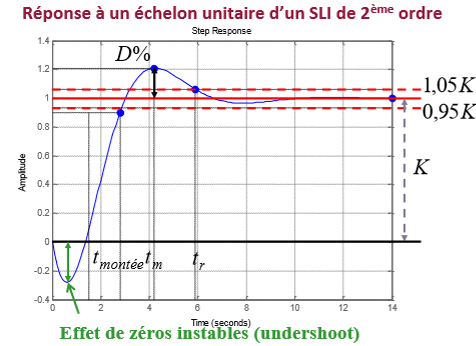
\includegraphics[scale=0.65]{Pics/SLI_Troubleshoot.png}
\end{center}
\newpage
\section{Retour d'état}
\begin{center}
    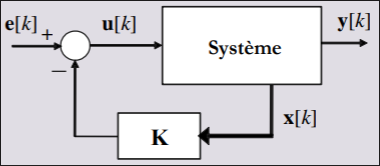
\includegraphics[scale=0.7]{Pics/retour_etat.png}
\end{center}
\subsection{Cas continu}
\large{Soit le système représenté en boucle ouverte :}
\begin{center}
    \fbox{\LARGE{$
    \dot x(t) = Ax(t) + Bu(t)
    $}} \newline 
    
    Avec : $x \in \mathbb{R}^{n}, u(t) \in \mathbb{R}$
\end{center}
\large{En boucle fermée, la commande par retour d'état impose \newline
$ u(t) = -Kx(t) + e(t)$, $e \in \mathbb{R}$. Il vient :}
\begin{center}
    \fbox{\LARGE{$
    \dot x(t) = (A - BK)x(t) + Be(t)
    $}}
\end{center}
\subsection{Cas discret}
\large{Soit le système représenté en boucle ouverte :}
\begin{center}
    \fbox{\LARGE{$
    x[k+1] = Fx[k] + Gu[k]
    $}} \newline 
    
    Avec : $x \in \mathbb{R}^{n}, u[k] \in \mathbb{R}$
\end{center}
\large{En boucle fermée, la commande par retour d'état impose \newline
$ u[k] = -Kx[k] + e[k]$, $e \in \mathbb{R}$. Il vient :}
\begin{center}
    \fbox{\LARGE{$
    x[k+1] = (F - GK)x[k] + Be[k]
    $}}
\end{center}
\newpage
\section{Calcul du retour d'état par placement des pôles}
\large{C'est le cacul de $K$ en choisissant les valeurs propres de $F - GK$. D'après le \textcolor{BrickRed}{théorème de Wonham : il existe une matrice K tq pour tout choix de valeurs propres SSI le système est totalement commandable.} \newline
(i.e. $\exists K \in M_{n}(\mathbb{R})$, on peut choisir les $\lambda_{i} \in S_{p}(A - BK)$ SII $\forall \lambda \in S_{p}(A), Re(\lambda) 0$)}
\subsection{Cas continu}
\begin{center}
    \fbox{\Large{$
x(t) = e^{(A - BK)(t-t_{0})}x(t_{0})
= \sum_{i=1}^{n}{\alpha_{i}e^{\lambda_{i}(t-t_{0})}}
$}} \footnote{$\lambda_{i}$ vp de $A - BK$ ($\lambda_{i} \in S_{p}(A-BK)$)}
\end{center}
\subsection{Cas discret}
\begin{center}
    \fbox{\Large{$
x[k] = (F - GK)^{k-k_{0}}x[k_{0}]
= \sum_{i=1}^{n}{\alpha_{i}\lambda_{i}^{(k-k_{0})}}
$}} \footnote{$\lambda_{i}$ vp de $F - GK$ ($\lambda_{i} \in S_{p}(F-GK)$)}
\end{center}
\subsection{Principe}
On cherche à avoir 
\[K = 
\begin{bmatrix}
    k_{1} & k_{2} & ... & k_{n}
\end{bmatrix}
\in \mathbb{R}^{n}
\]
tel que $\forall i \in \{1,n\}$, les $k_{i}$ sont les pôles de la fonction de transfert du système et les critères de commandabilité sont respectés soit :
\begin{center}
    \item $\forall \lambda_{i} \in S_{p}(A - BK),Re(\lambda_{i}) < 0$ \newline
\end{center} 

\newpage
\subsection{Calcul de $K$}
On veut choisir les $\lambda_{i}$ tel que $|\lambda I - (A - BK)| = \prod_{i=1}^{n}(\lambda - \lambda_{i})$ \newline
\begin{itemize}
    \item \textcolor{BrickRed}{Formule d'Ackerman} (si $dim(u) = 1$) : \newline
    \begin{itemize}
        \item \Large{$
            (\lambda - \lambda_{1})(\lambda - \lambda_{2})(\lambda - \lambda_{3})...(\lambda - \lambda_{n}) = \lambda^{n} + \alpha_{1}\lambda^{n-1} + ... + \alpha_{n-1}\lambda + \alpha_{n}
            $} \newline
        \item \Large{$
        P(A) = A^{n} + \alpha_{1}A^{n-1} + ... + \alpha_{n-1}A + \alpha_{n}I_{n} 
        $} \newline
        \item Soit : \newline
        \Large{$
        K = [ 0  0  ...  0  1 ][B | AB | A^{2}B | ... | A^{n-1}B]P(A)
        $} \newline
    \end{itemize}
    \item \textcolor{BrickRed}{Calcul à partir des valeurs propres} ($dim(u) quelconque$) \newline
    \begin{itemize}
        \item Trouver les $(v_{i})_{i \in \llbracket 1 , n \rrbracket}$ et $(w_{i})_{i \in \llbracket 1 , n \rrbracket}$ tel que : \newline
        \Large{$
        \forall i \in \llbracket 1 , n \rrbracket , (A - \lambda_{i}I_{n})v_{i} - Bw_{i} = 0_{n}
        $} \newline
        \item Soit : 
    \[K = 
    \begin{bmatrix}
        v_{1} & ... & v_{n}
    \end{bmatrix}
    \begin{bmatrix}
        w_{1} & ... & w_{n}
    \end{bmatrix}
    ^{-1}\]
    \end{itemize}
\end{itemize}
\subsection{Critères à respecter pour le choix des $\lambda_{i}$}
\begin{itemize}
    \item $\forall \lambda_{i} \in S_{p}(A - BK),Re(\lambda_{i} 0)$ \newline
    \item Les pôles dominants sont tels que $\forall \lambda_{i} \in S_{p}(A - BK), \newline
    \lambda_{dominant} = max_{i \in \llbracket 1 , n \rrbracket}(Re(\lambda_{i}))$ \footnote{Pour un système stable} \newline
    \item Plus les $\lambda_{i}$ sont éloignés des vp de A, plus les amplitudes des gains de $K$ et donc des commandes $u(t)$ sont forte
\end{itemize}
\newpage
\subsection{Exemple pour la formule d'Ackerman}
On considère une fonction de transfert d'ordre 2 tel que : 
\begin{center}
    \Large{$
        H(p) = \frac{K}{(p - p_{1})(p - p_{2})}
    $}
\end{center}
Avec $p_{1}$ et $p_{2}$ les pôles de la fonctionde transfert. On veut :  
\[
K = 
\begin{bmatrix}
    p_{1} & p_{2}
\end{bmatrix}
\] tel que : 
\begin{center}
\fbox{\Large{$
    |\lambda I_{2} - (A - BK) | = (\lambda - p_{1})(\lambda - p_{2}) = \lambda^{2} + 2\xi \omega_{0}\lambda + \omega_{0}^{2} 
$}}
\end{center}
\textbf{1.} On procède par identification :
\[
    \left \{
    \begin{array}{c @{=} c}
        1 & 1 \\
        2\xi \omega_{0} & -p_{1} - p_{2}\\
        \omega_{0}^{2} & p_{1}p_{2} 
    \end{array}
    \right.
\]
\textbf{2.} Les $\xi$ et $\omega_{0}$ sont trouvés grâce aux équations suivantes : 
\begin{center}
    \fbox{\Large{$
    D = e^{-\frac{\pi \xi}{\sqrt{1-\xi^{2}}}}
    $}}
\end{center}
    \begin{center}
    \fbox{\Large{$
    t_{m} = \frac{\pi}{\omega_{0}\sqrt{1-\xi^{2}}}
    $}} \footnote{Avec : \Large{$
    \omega_{0}t_{m} =  3
    $}}
\end{center}
\textbf{3.} En résolvant le système d'équations, on trouve la valeur des pôles de $K$ \newline

Pour une FT d'ordre 3, on considère :
\[
K = 
\begin{bmatrix}
    p_{1} & p_{2} & p_{3}
\end{bmatrix}
\]
On a alors l'équation suivante :
\begin{center}
    \Large{$
    |\lambda I_{3} - (A - BK) | = (\lambda - p_{1})(\lambda - p_{2})(\lambda - p_{3}) = \lambda^{3} + 2\xi \omega_{0}\lambda^{2} + 2\alpha \omega_{0}^{2}\lambda + \omega_{0}^{3} 
    $}    
\end{center}
Comme la valeur $\alpha$ n'est pas atteignable, ce système est résolu à l'aide de fonctions Matlab telles que \texttt{place}. \textbf{Pour une résolution complète, voir suspension EM, cours CSD03}.
\newpage
\section{Calcul du gain statique}
On ajoute un gain $k_{c}$ en entrée de boucle :
\begin{center}
    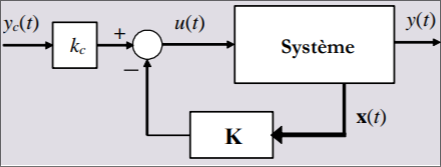
\includegraphics[scale=0.5]{Pics/retour_etat_KC.png}
\end{center}
De manière à satisfaire le critère de précision ($\epsilon_{s} = 0$) du
système bouclé : 
\subsubsection{Cas continu}
\Large{
    \[
\left \{
\begin{array}{c @{=} c}
    \dot x(t) & (A - BK)x(t) + Bk_{c}y_{c}(t)\\
    y(t) & Cx(t)
\end{array}
\right.
\]
\large{
Avec : $dim(y) = dim(u) = 1$\newline
En régime permettant, on veut $y(t) = y_{c}(t) = y_{c}$ \newline
Soit :}
\begin{center}
    \fbox{\Large{$
    k_{c} = \frac{-1}{C(A-BK)^{-1}B}
    $}}
\end{center} 
\subsubsection{Cas discret}
\Large{
\[
\left \{
\begin{array}{c @{=} c}
    x[k+1] & (F - GK)x[k] + Gk_{c}y_{c}[k]\\
    y[k] & Cx[k]
\end{array}
\right.
\]
\large{
Avec : $dim(y) = dim(u) = 1$\newline
En régime permettant, on veut $y(t) = y_{c}(t) = y_{c}$ \newline
Soit :}
\begin{center}
    \fbox{\Large{$
    k_{c} = \frac{-1}{C(I_{n}-F + GK)^{-1}G}
    $}}
\end{center} 
\footnote{Attention : l'erreur statique est non nulle si la perturbation est constante}
\subsection{perturbation constante et mesurable}
\large{
Ici, on cherche à modéliser l'influence d'une perturbation sur un système bouclé avec un gain statique determiné, de façon à mettre en évidence la remarque émise sur la page précédente.
\begin{center}
    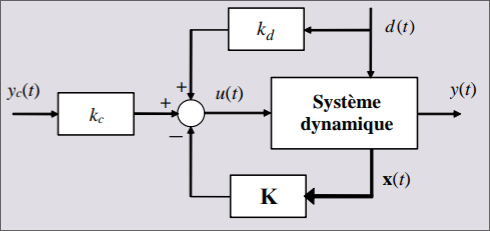
\includegraphics[scale=0.5]{Pics/Perturbations.png}
\end{center}
\large{Système en boucle fermée :}
}
\Large{
    \[
\left \{
\begin{array}{c @{=} c}
    \dot x(t) & Ax(t) + Bu(t) + B'd(t)\\
    y(t) & Cx(t)
\end{array}
\right.
\]
\large{Commande :} \newline
$u(t) = -Kx(t) + k_{c}y_{c}(t) + k_{d}d(t)$
\large{système en boucle ouverte :}
\Large{
    \[
\left \{
\begin{array}{c @{=} c}
    \dot x(t) & (A - BK)x(t) + Bk_{c}y_{c}(t) + (Bk_{d} + B')d(t)\\
    y(t) & Cx(t)
\end{array}
\right.
\]
\large{En régime permettant, on veut toujours $y(t) = y_{c}(t) = y_{c}$ \newline
Soit :}
\Large{
    \[
\left \{
\begin{array}{c @{=} c}
    k_{c} & -[C(A - BK)^{-1}B]^{-1}\\
    k_{d} & -[C(A - BK)^{-1}B]^{-1}[C(A - BK)^{-1}B']
\end{array}
\right.
    \]}
\newpage
\subsection{Exemple : suspension magnétique}
On considère le système suivant :
\begin{figure}[hbt!]
    \centering
    \begin{subfigure}{.5\textwidth}
      \centering
      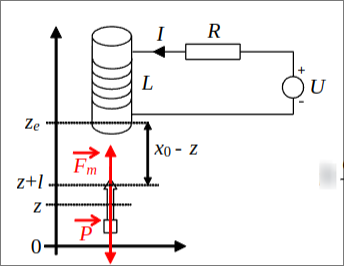
\includegraphics[width=1\linewidth]{Pics/suspension_magnetique.png}
      \caption{Schéma associé au système}
      \label{fig:sub1}
    \end{subfigure}%
    \begin{subfigure}{.7\textwidth}
      \centering
      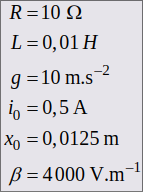
\includegraphics[width=.4\linewidth]{Pics/AN_suspension_magnetique.png}
      \caption{Application numérique}
      \label{fig:sub2}
    \end{subfigure}
    \caption{Sytème}
    \label{fig:test}
\end{figure}
\begin{center}
    \Large{$
    L\frac{dI(t)}{dt} + RI(t) = U(t)
    $} \footnote{Loi des mailles}
    \newline

    \Large{$
    m\frac{d^{2}z}{dt} = c\frac{I(t)}{(x_{0} - z(t)^{2}} - mg = F_{m} - mg
    $} \footnote{PFD}
\end{center}
\large{
\textbf{Point d'équilibre $\overline{z} = 0$}
}
\large{
    \[
\left \{
\begin{array}{c @{=} c}
    \overline{U} & R\overline{I} \\
    c\frac{\overline{I}}{x_{0}^{2}} - mg & 0
\end{array}
\right.
\]}
soit :
\large{
    \[
\left \{
\begin{array}{c @{=} c}
    \overline{I} & \frac{mgx_{0}^{2}}{c} = i_{0} \\
    \overline{U} & R\overline{I} = Ri_{0}
\end{array}
\right.
    \]}
En linéarisant sur le point d'équilibre, on a :
\large{
    \[
    \left \{
\begin{array}{c @{=} c}
    I(t) & \overline{I} + i_{1}(t) \\
    U(t) & \overline{U} + u_{0}(t)
\end{array}
\right.
    \]}
\newpage
Equations du système :
\begin{center}
    \Large{$
    L\frac{di_{1}(t)}{dt} + Ri_{1}(t) = u_{1}(t)
    $} 
    \newline

    \Large{$
    m\frac{d^{2}z}{dt} = g\frac{i_{1}(t)}{(i_{0}} + \frac{2g}{x_{0}}z(t)
    $}
    \newline

    \Large{$
    V_{z}(t) = \beta z(t)
    $} \footnote{Mesures : $V_{z}(t)$ et $i_{1}(t)$}
\end{center}
Le vecteur d'état s'écrit : 
\begin{center}
    \[
    x(t) = 
    \begin{bmatrix}
    i_{1}(t) \\
    z(t) \\
    \dot{z}(t)    
    \end{bmatrix}
    \]
\end{center}
\textbf{Représentation d'état}
\begin{center}
    \[
    \frac{d}{dt}
    \begin{bmatrix}
    i_{1}(t) \\
    z(t) \\
    \dot{z}(t)    
    \end{bmatrix}
    =
    \begin{bmatrix}
        -1000 & 0    & 0 \\
        0     & 0    & 1 \\
        20    & 1600 & 0
    \end{bmatrix}
    \begin{bmatrix}
        i_{1}(t) \\
        z(t) \\
        \dot{z}(t)    
    \end{bmatrix}
    +
    \begin{bmatrix}
        100 \\
        0 \\
        0
    \end{bmatrix}
    \] \newline
    \[
    V_{z}(t) = 
    \begin{bmatrix}
        0 & 4000 & 0
    \end{bmatrix}
    \begin{bmatrix}
        i_{1}(t) \\
        z(t) \\
        \dot{z}(t)    
    \end{bmatrix}
    \]
\end{center}
\newpage
\textbf{Analyse en boucle ouverte}
\newline
\begin{itemize}
    \item \textbf{Stabilité :} Calcul des valeurs propres de A \newline
    \begin{center}
        $S_{p}(A) = \{-1000;-40;\textcolor{BrickRed}{40}\} \implies$ le système est instable
    \end{center} 
    \item \textbf{commandabilité : } Calcul de la matrice de commandabilité \newline
    \begin{center}
        \[
        Q_{c} = 
        \begin{bmatrix}
            B & AB & A^{2}B
        \end{bmatrix}
        =
        \begin{bmatrix}
            100 & -10^{5} & 10^{8} \\
            0   & 0       & 2.10^{3} \\
            0   & 2.10^{3}& -2.10^{6}
        \end{bmatrix}
        \]
        \newline
        $
        rg(Q_{c}) = 3 \implies
        $ le système est commandable
    \end{center}
    \item \textbf{Observabilité : } calcul de la matrice d'observabilité $Q_{0}$
    \begin{center}
        \[
        Q_{0} = 
        \begin{bmatrix}
            C \\
            CA \\
            CA^{2}
        \end{bmatrix}
        =
        \begin{bmatrix}
            0       & 4.10^{3}  & 0 \\
            0       & 0         & 4.10^{3} \\
            8.10^{4}& 6,4.10^{6}& 0
        \end{bmatrix}
        \]
        \newline
        $
        rg(Q_{0}) = 3 \implies
        $ le système est observable
    \end{center}    
\end{itemize}
\textbf{Système en boucle ouverte}
\begin{center}
    \[
    \frac{d}{dt}
    \begin{bmatrix}
    i_{1}(t) \\
    z(t) \\
    \dot{z}(t)    
    \end{bmatrix}
    =
    \begin{bmatrix}
        -1000 & 0    & 0 \\
        0     & 0    & 1 \\
        20    & 1600 & 0
    \end{bmatrix}
    \begin{bmatrix}
        i_{1}(t) \\
        z(t) \\
        \dot{z}(t)    
    \end{bmatrix}
    +
    \begin{bmatrix}
        100 \\
        0 \\
        0
    \end{bmatrix}
    \] \newline
    \[
    V_{z}(t) = 
    \begin{bmatrix}
        0 & 4000 & 0
    \end{bmatrix}
    \begin{bmatrix}
        i_{1}(t) \\
        z(t) \\
        \dot{z}(t)    
    \end{bmatrix}
    \] \newline
    \[
    u_{1}(t) = -Kx(t) + k_{c}y_{c}(t) =
    \begin{bmatrix}
        k_{1} & k_{2} & k_{3}
    \end{bmatrix}
    \begin{bmatrix}
        i_{1}(t) \\
        z(t) \\
        \dot{z}(t)    
    \end{bmatrix}
    + k_{c}y_{c}(t)
    \] \footnote{Commande par retour d'état (bouclage)}
\end{center}
\newpage
\textbf{Système bouclé} \footnote{On injecte l'expression de $u_{1}$}
\begin{center}
    \[
    \frac{d}{dt}
    \begin{bmatrix}
    i_{1}(t) \\
    z(t) \\
    \dot{z}(t)    
    \end{bmatrix}
    =
    \begin{bmatrix}
        -1000-100k_{1} & -100k_{2}  & -100k_{3} \\
        0              & 0          & 1         \\
        20             & 1600       & 0
    \end{bmatrix}
    \begin{bmatrix}
        i_{1}(t) \\
        z(t) \\
        \dot{z}(t)    
    \end{bmatrix}
    +
    \begin{bmatrix}
        100k_{c} \\
        0 \\
        0
    \end{bmatrix}
    y_{c}(t)
    \] \newline
    \[
        V_{z}(t) = 
        \begin{bmatrix}
            0 & 4000 & 0
        \end{bmatrix}
        \begin{bmatrix}
            i_{1}(t) \\
            z(t) \\
            \dot{z}(t)    
        \end{bmatrix}
    \]
\end{center}
\textbf{Cahier des charges} \newline
On cherche maintenant à remplir le cahier des charges suivant :
\[
    \left \{
    \begin{array}{c @{=} c}
        D & 10\%\\
        t_{m} & 0.03s
    \end{array}
    \right.
\]
Ce qui donne :
\[
    \left \{
    \begin{array}{c @{=} c}
        \xi & 0.6\\
        \omega_{0} & 130
    \end{array}
    \right.
\]
Comme les valeurs propres de $A$ ne vérifient pas le critère de stabilité (40 a une partie réelle positive), on choisit alors comme valeurs
propres -1000 et deux valeurs : $\omega$ et $\xi$ déterminés grâce au cahier des charges 
\footnote{
    Les $\xi$ et $\omega_{0}$ sont trouvés grâce aux équations suivantes : 
    \begin{center}
        \fbox{\Large{$
        D = e^{-\frac{\pi \xi}{\sqrt{1-\xi^{2}}}}
        $}}
    \end{center}
    \begin{center}
        \fbox{\Large{$
        t_{m} = \frac{\pi}{\omega_{0}\sqrt{1-\xi^{2}}}
        $}} 
        Avec : \Large{$
        \omega_{0}t_{m} =  3
        $}
    \end{center}
}
en résolvant le système d'équations}
. \large{On résoud alors l'équation :}
\begin{center}
    \large{$
        |\lambda I_{3} - (A - BK)| = (\lambda + 1000)(\lambda^{2} + 2*0.6*130*\lambda + 130^{2})
    $}
\end{center}
\textbf{Placement des pôles} \newline
Grâce à la fonction \texttt{place} de Matlab (par \textbf{identification}): 
\begin{center}
    \large{$
    k_{1} = 1,560; k_{2} = 9,375.10^{3}; k_{3} = 87,25
    $}
\end{center}
\newpage
\textbf{Calcul de $k_{c}$}
\begin{center}
    \[
    \frac{d}{dt}
    \begin{bmatrix}
    i_{1}(t) \\
    z(t) \\
    \dot{z}(t)    
    \end{bmatrix}
    =
    \begin{bmatrix}
        -1000-100k_{1} & -100k_{2}  & -100k_{3} \\
        0              & 0          & 1         \\
        20             & 1600       & 0
    \end{bmatrix}
    \begin{bmatrix}
        i_{1}(t) \\
        z(t) \\
        \dot{z}(t)    
    \end{bmatrix}
    +
    \begin{bmatrix}
        100k_{c} \\
        0 \\
        0
    \end{bmatrix}
    y_{c}(t)
    \] \newline
    \[
    V_{z}(t) = 
    \begin{bmatrix}
        0 & 4000 & 0
    \end{bmatrix}
    \begin{bmatrix}
        \overline{i_{1}} \\
        \overline{z} \\
        \overline{\dot{z}}   
    \end{bmatrix}
    \]
\end{center}
A l'équilibre
\begin{center}
    \[
    \begin{bmatrix}
    0 \\
    0 \\
    0    
    \end{bmatrix}
    =
    \begin{bmatrix}
        -1000-100k_{1} & -100k_{2}  & -100k_{3} \\
        0              & 0          & 1         \\
        20             & 1600       & 0
    \end{bmatrix}
    \begin{bmatrix}
        \overline{i_{1}} \\
        \overline{z} \\
        \overline{\dot{z}}   
    \end{bmatrix}
    +
    \begin{bmatrix}
        100k_{c} \\
        0 \\
        0
    \end{bmatrix}
    \overline{y_{c}}
    \] \newline
    \[
    V_{z}(t) = 
    \begin{bmatrix}
        0 & 4000 & 0
    \end{bmatrix}
    \begin{bmatrix}
        \overline{i_{1}} \\
        \overline{z} \\
        \overline{\dot{z}}  
    \end{bmatrix}
    \]
\end{center}
Soit : 
\[
    \left \{
    \begin{array}{c @{=} c}
        \overline{k_{c}} = \frac{1000+100k_{1}\overline{i_{1}} + 100k_{2}\overline{z} + 100k_{3}\overline{\dot{z}}}{100y_{c}} \\
        \overline{\dot{z}} & 0 \\
        \overline{y_{c}} & -\overline{z}\\
        \overline{V_{z}} & 4000 \overline{z} = - \frac{4000k_{c}}{800 +80k_{1}-k_{2}}\overline{y_{c}} 
    \end{array}
    \right.
\]
Or on veut que l'érreur statique soit nulle ($\epsilon_{s} = 0$). On a alors : 
\begin{center}
    \LARGE{$
    -\frac{4000k_{c}}{800 + 80k_{1}-k_{2}} = 1 \Longleftrightarrow k_{c} = -\frac{800 +80k_{1}-k_{2}}{4000} = 2.125
    $} 
    \textcolor{white}{.}\newline
    \footnote{justifiable par le théorème de la valeur finale, on veut finalement que $\frac{S(p)}{E(p)}=1$}
\end{center}
\newpage
\section{Commande par retour d'état des systèmes partiellment commandables}
\large{système en boucle ouverte :}
\[
\begin{bmatrix}
   \dot{x_{1}}(t) \\
   \dot{x_{2}} 
\end{bmatrix}
 = 
\begin{bmatrix}
    A_{11} & A_{12} \\
    0      & A_{22}
\end{bmatrix}
\begin{bmatrix}
    \dot{x_{1}(t)} \\
    \dot{x_{2}} 
\end{bmatrix}
+
\begin{bmatrix}
    B_{1} \\
    0
\end{bmatrix}
u(t)
\]
\large{Commande par retour d'état :}\newline
\[ u(t) = 
 - \begin{bmatrix}
   K_{1} & K_{2}
\end{bmatrix}
x(t) + e(t)
\]
\large{Boucle fermée :} \newline
\[
\begin{bmatrix}
   \dot{x_{1}}(t) \\
   \dot{x_{2}}(t) 
\end{bmatrix}
 = 
\begin{bmatrix}
    A_{11} - B_{1}K_{1} & A_{12} - B_{1}K_{2} \\
    0                   & A_{22}
\end{bmatrix}
x(t) + Be(t)
\]
\newpage
\section{Commande modale}
\subsection{Opérateur $q$}
\large{L'opérateur $q$ désigne l'opérateur dérivée, de telle sorte que l'on ai :}
\subsubsection{Cas continu}
\begin{center}
    \Large{\fbox{$
    \forall \vec{x} \in R^{n}, q\vec{x}(t) = \frac{d\vec{x}(t)}{dt}
    $}}
\end{center}
\subsubsection{Cas discret}
\begin{center}
    \Large{\fbox{$
    \forall \vec{x} \in R^{n}, q\vec{x}[n] = \vec{x}[n+1]
    $}}
\end{center}
\subsection{Variable $q$}
\large{$q$ en tant que variable \textbf{complexe} désigne $p$ ou $z$ selon le domaine}
\subsection{Principe}
\large{La commande modale consiste à considérer une nouvelle entrée e telle que :}
\begin{center}
    \Large{$
    \vec{u} = \vec{e} - K\vec{x}
    $}
\end{center}
\large{Ce qui donne comme nouvelle représentation d'état : }
\begin{center}
    \Large{
    \[
        \left \{
        \begin{array}{c @{=} c}
            q\vec{x} & (A - BK)\vec{x} + B\vec{e}\\
            \vec{y} & (C - DK)\vec{x} + D\vec{e}
        \end{array}
        \right.
    \]
    }
\end{center}
\large{Fonction de transfert : }
\begin{center}
    \Large{$
    H(q) = [(C - DK)(qI_{n} - (A - BK))^{-1}B + D]E(q)
    $}\footnote{Attention : ici $q$ désigne la variable complexe dans le domaine de Laplace ou de la transformée en $Z$ ($q = p$ dans le domaine de Lapalce et $q = z$ pour la transformée en $Z$)}
\end{center}
\newpage
\section{Modification des pôles de la fonction de transfert}
\large{Critère de la matrice de commandabilité}
$N = rg(Q_{c})$\footnote{$N$ : nombre de pôles modifiables} avec :
\[
Q_{c} = 
\begin{bmatrix}
    B & AB & A^{2}B & ... & A^{n-1}B
\end{bmatrix}
\]

\begin{itemize}
    \item Exprimer $\chi_{A - BK}(q) = |qI_{n} - (A - BK)| = q^{n} + \sum_{k=0}^{n-1}{a_{k}q^{k}}$ en fonction des valeurs inconnues de $K$
    \item Par identification, trouver les éléments de $K$ (système d'équations) à partir des $(a_{k})_{k \in N}$ et des pôles choisis arbitrairements
\end{itemize}
A COMPLETER
\newpage
\section{Commande LQ}
\subsection{Principe}
\large{Pour un système tel que :}
\[
    \left \{
    \begin{array}{c @{=} c}
        \dot x(t) & Ax(t) + Bu(t)\\
        u(t) & -Kx(t)
    \end{array}
    \right.
\]
\large{de condition initiale $x(0) = x_{0}$, on cherche $K$ qui minimise un des critères de performance $J$ :\footnote{Soit $u$ tel que $\forall x_{0}$ qui minimise le critère} }
\begin{itemize}
    \item Temps de réponse
    \item Temps de dépassement
    \item Amplitude du premier dépassement
    \item Erreur statique
    \item ...
\end{itemize}
\large{Représenté par :}
\begin{center}
    \Large{\fbox{$
    K = min(J) = min(\int_{0}^{+\infty}{
        x(t)^{T}Qx(t) + u(t)^{T}Ru(t)
        })
    $}} OU
    \newline
    \Large{\fbox{$
    K = min(J) = min(\sum_{k=0}^{+\infty}{
        x[k]^{T}Qx[k] + u[k]^{T}Ru[k]
        })
    $}}
\end{center}
\large{Avec : $Q^{T} = Q$ et $R^{T} = R$}
\subsection{Solution}
$\exists$ une solution $(A,B)$ \textbf{stabilisable}, $(H,A)$ \textbf{détectable} avec $H$ tel que $Q = H^{T}H$, la matrice $P^{T} = P$ unique solution positive de \textbf{l'équation algébrique de Riccati} : 
\begin{center}
    \Large{\fbox{$
    PA + A^{T}P - PBR^{-1}B^{T}P + Q = 0_{n}
    $}}
\end{center}
\large{tel qu'on ai :}
\begin{center}
    \Large{\fbox{$
    K = -R^{-1}B^{T}P
    $}}
\end{center}
Avec :
\begin{center}
    \Large{$
    \dot{x}(t) = Ax(t) + Bu(t)
    $} en boucle ouverte
    \Large{{$
    u(t) = -Kux(t)
    $}} en boucle fermée
\end{center}
\newpage
\begin{itemize}
    \item Démarche de réglage des pondérations
    \begin{itemize}
        \item Normalisation des variables
        \item Limitation du nombre de coefficients et prévisions de leurs influence $\longrightarrow$ Matrices de pondération diagonale
        \item Itérations à partir du choix initial
        \begin{itemize}
            \item \textcolor{BrickRed}{Si éléments de $Q$ $\nearrow$, Rapidité $\nearrow$}
            \item \textcolor{BrickRed}{Si éléments de $R$ $\nearrow$, Rapidité $\searrow$} 
        \end{itemize}
        \begin{itemize}
            \item \textcolor{BrickRed}{Si éléments de $Q$ $\nearrow$, Stabilité $\nearrow$}
            \item \textcolor{BrickRed}{Si éléments de $R$ $\nearrow$, Stabilité $\nearrow$} 
            \item \textcolor{BrickRed}{Attention : si le rapport $\frac{Q}{R}$ est trop élevé, stabilité $\searrow$}
        \end{itemize}
    \end{itemize}
\end{itemize}
\subsection{Commande LQ à l'horizon infini - cas continu}
Pour un système :
\begin{center}
    \Large{
        \[
        \left \{
        \begin{array}{c @{=} c}
            \dot x(t) & Ax(t) + Bu(t)\\
            y(t) & Cx(t)
        \end{array}
        \right.
        \]
    }
\end{center}
Choix du critère : 
\begin{center}
    \Large{$
        J = \int_{0}^{+\infty}{
        y(t)^{T}\tilde{Q}y(t) + u(t)^{T}Ru(t)
        }
    $} Avec : 
    \Large{$
    Q = C^{T}\tilde{Q}C
    $}
\end{center}
\begin{center}
    \Large{
        \fbox{$u(t) = -Kx(t)$}
    }
    Avec : 
    \begin{center}
        $K = (R + B^{T}PB)^{-1}B^{T}PA$, \newline
        $P = Q + A^{T}PA - A^{T}PB(R + B^{T}PB)^{-1}B^{T}PA$ \footnote{Equation de Riccati}
    \end{center}
\end{center}
\textbf{Pour un exemple de commande LQ, voir Commande LQ, cours CSD04}
\newpage
\subsection{Exemple : mouvement latéral d'un avion}
\textbf{Représentation d'état}
\begin{center}
    \[
    \frac{d}{dt}
    \begin{bmatrix}
    \beta (t) \\
    p(t) \\
    r(t) \\
    \phi (t)    
    \end{bmatrix}
    =
    \begin{bmatrix}
        -0,75 & 0,006  & -1    & 0,0037 \\
        -12,9 & -0,75  & 0,387 & 0      \\
        4,31  & 0,0024 & -0,17 & 0      \\
        0     & 1      & 0     & 0
    \end{bmatrix}
    \begin{bmatrix}
        \beta (t) \\
        p(t) \\
        r(t) \\
        \phi (t)    
    \end{bmatrix}
    +
    \begin{bmatrix}
        0,0012 & 0,0092 \\
        6,05   & 0,952  \\
        -0,416 & -1,76  \\
        0      & 0 
    \end{bmatrix}
    \begin{bmatrix}
        \delta_{a}(t) \\
        \delta_{d}(t)
    \end{bmatrix}
    \]
\end{center}
\textbf{Cahier des charges}
`\begin{itemize}
    \item Temps de réponse à 5\% inférieur à $3s$
    \item Amplitude de dépassement raisonable
    \item Amortissement raisonable
\end{itemize}
\textbf{Critère}
\begin{center}
    \Large{$
    J = \int_{0}^{\infty}(q_{1}\beta^{2}(t) + q_{2}\phi^{2}(t) + r_{1}\delta_{a}^{2}(t) + r_{2}\delta_{d}^{2}(t)){dt}
    $}
\end{center}
\begin{figure}[hbt!]
    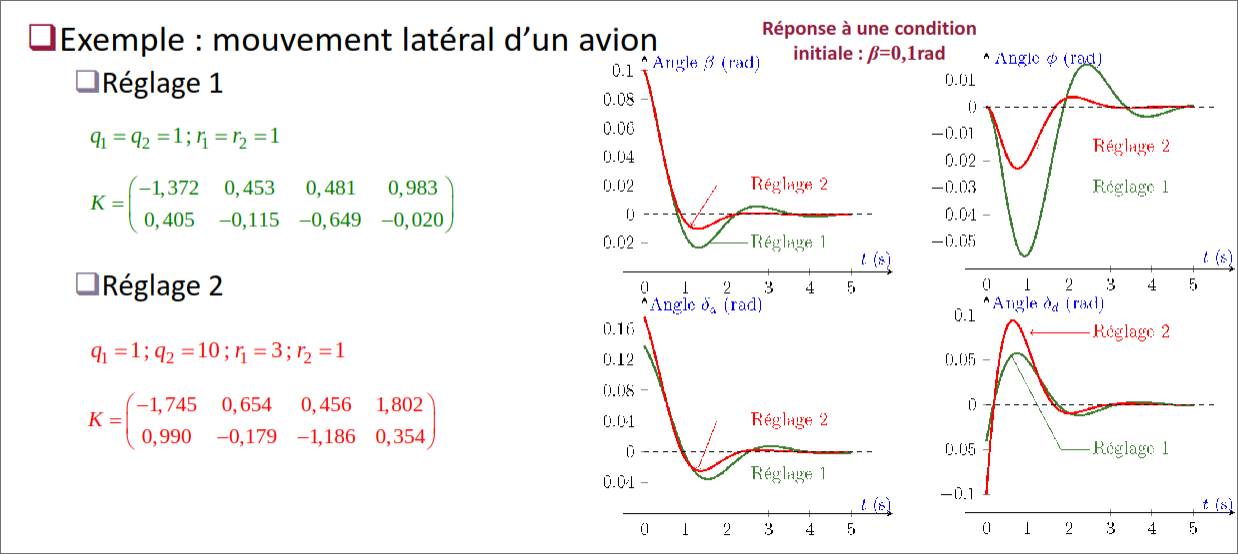
\includegraphics[scale=0.25]{Pics/reglage1_LQ.png}
    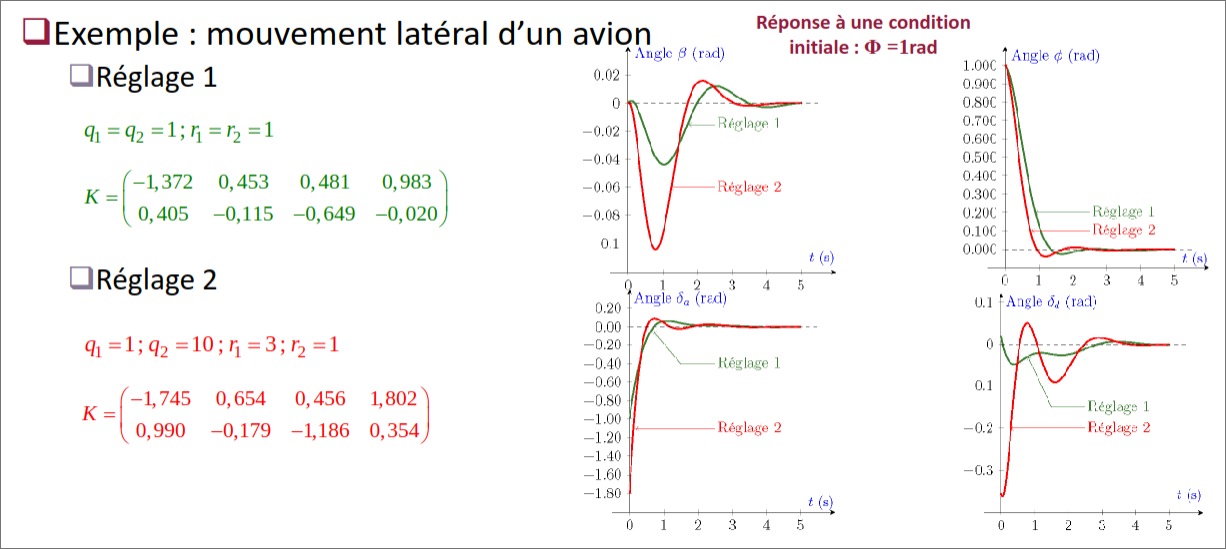
\includegraphics[scale=0.25]{Pics/reglage2_LQ.png}
\end{figure}
\newpage
\section{Commande à action intégrale}
\subsection{Principe}
\begin{figure}[hbt!]
    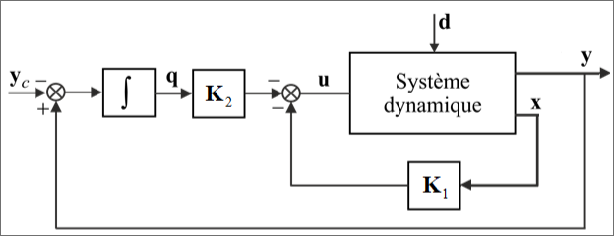
\includegraphics[scale=0.5]{Pics/commande_action_integrale.png}
\end{figure}
Représentation d'état en boucle ouverte :
\Large{
    \[
\left \{
\begin{array}{c @{=} c}
    \dot x(t) & Ax(t) + Bu(t) + B'd(t)\\
    y(t) & Cx(t)
\end{array}
\right.
\]
\large{
\textbf{L'objectif est d'asservir $y(t)$ sur $y_{c}(t) = y_{c}$ malgrès la perturbation $d(t) = d$ constante}
Action integrale : }
\begin{center}
    \Large{\fbox{$
    q(t) = \int_{0}^{t}(y(\tau) - y_{c}){d\tau}
    $}}
\end{center}
On inclus alors dans la représentation d'état l'action intégrale $q$, appelé \textbf{système augmenté} : 
\begin{center}
    \[
    \frac{d}{dt}
    \begin{bmatrix}
        x(t) \\
        q(t)
    \end{bmatrix}
    =
    \begin{bmatrix}
        A & 0_{n} \\
        C & 0_{n}
    \end{bmatrix}
    \begin{bmatrix}
        x(t) \\
        q(t)
    \end{bmatrix}
    +
    \begin{bmatrix}
        B \\
        0_{n}
    \end{bmatrix}
    u(t) +
    \begin{bmatrix}
        B' & 0_{n} \\
        0_{n} & - I_{n}
    \end{bmatrix}
    \begin{bmatrix}
        d(t) \\
        y_{c}(t)
    \end{bmatrix}
    \] \newline
    \[
    y(t) = 
    \begin{bmatrix}
        C & 0_{n}
    \end{bmatrix}
    \begin{bmatrix}
        x(t) \\
        q(t)
    \end{bmatrix}
    \]
\end{center}
Soit : 
\Large{
    \[
\left \{
\begin{array}{c @{=} c}
    \dot x_{a}(t) & A_{a}x_{a}(t) + B_{a}u(t) + B'_{a}d_{a}(t)\\
    y_{a}(t) & C_{a}x_{a}(t)
\end{array}
\right.
\]
\newpage
\large{\textbf{Commande par retour d'état}} 
\begin{center}
    \Large{$
    u(t) = -Kx_{a}(t) =  -K_{1}x(t) - K_{2}q(t)
    $}
    \newline
    \[
    K = 
    \begin{bmatrix}
        k_{1,1} &  ... & k_{1,n} & k_{2,1} & ... & k_{2,n}
    \end{bmatrix}
    , x_{a}(t) = 
    \begin{bmatrix}
        x_{1}(t) \\
        ...      \\
        x_{n}(t) \\
        q_{1}(t) \\
        ...      \\
        q_{n}(t)
    \end{bmatrix}
    \] 
\end{center}
On réalise une approche : 
\begin{itemize}
    \item \textbf{modale} si $(A_{a},B_{a})$ commandable \newline
    \item \textbf{LQ} si $(A_{a},B_{a})$ stabilisable et $(H,A_{a})$ détectable avec \newline 
        \begin{center}
            \begin{itemize}
                \item \Large{$
                    J = \int_{0}^{+\infty}{
                    y(t)^{T}\tilde{Q}y(t) + u(t)^{T}Ru(t)
                    }
                $} \newline
                \item \Large{$
                Q = H^{T}H
                $}
            \end{itemize}
        \end{center}
\end{itemize}

\large{\textbf{Action d'anticipation de la consigne}} \newline

\Large{$
u(t) = -Kx_{a}(t) =  -K_{1}x(t) - K_{2}q(t) + K_{c}y_{c}(t)
$} \newline

\large{\textbf{En régime permanent}} \newline

\begin{center}
    \[
    \begin{bmatrix}
        0_{\mathbb{R}^{n}} \\
        y_{c}
    \end{bmatrix}
    =
    \begin{bmatrix}
        A & B \\
        C & 0_{n}
    \end{bmatrix}
    \begin{bmatrix}
        x_{c} \\
        u_{c}
    \end{bmatrix}
    \]
\end{center}
Soit :
\begin{center}
    \[
    u_{c} = 
    \begin{bmatrix}
        0 & I_{n}
    \end{bmatrix}
    \begin{bmatrix}
        A & B \\
        C & 0_{n}
    \end{bmatrix}
    ^{-1}
    \begin{bmatrix}
        0_{n} \\
        I_{n}
    \end{bmatrix}
    y_{c}
    = K_{c}y_{c}
    \]
\end{center}